
\lstinputlisting[language=bash,basicstyle=\small]{python_codes/fieldstone_30/keywords}

\begin{center}
Code at \url{https://github.com/cedrict/fieldstone/tree/master/python_codes/fieldstone_30}
\end{center}

\par\noindent\rule{\textwidth}{0.4pt}
%%%%%%%%%%%%%%%%%%%%%%%%%%%%%%%%%%%%%%%%%%%%%%%%%%%%%%%%%%%%%%%%%%%%%%%%%%%%%%%%%%%%%%%%%%%5

In this the Stokes equations are not solved. It is a 2D implementation of the cvi algorithm 
as introduced in \cite{waav15} which deals with the advection of particles. 
$Q_1$ and $Q_2$ basis functions are used and in both cases the cvi algorithm can be toggled on/off. 
Particles can be distributed regularly or randomly at startup.

Three velocity fields are prescribed on the mesh:
\begin{itemize}
\item the so-called Couette flow of \cite{waav15} 
\item the SolCx solution (see Section~\ref{sec:geobench}, and  other stones too)
\item a flow created by means of a stream line function (see fieldstone 32)
\end{itemize}

%%%%%%%%%%%%%%%%%%%%%%%%%%%%%%%5
\subsection*{Couette flow}

\begin{center}
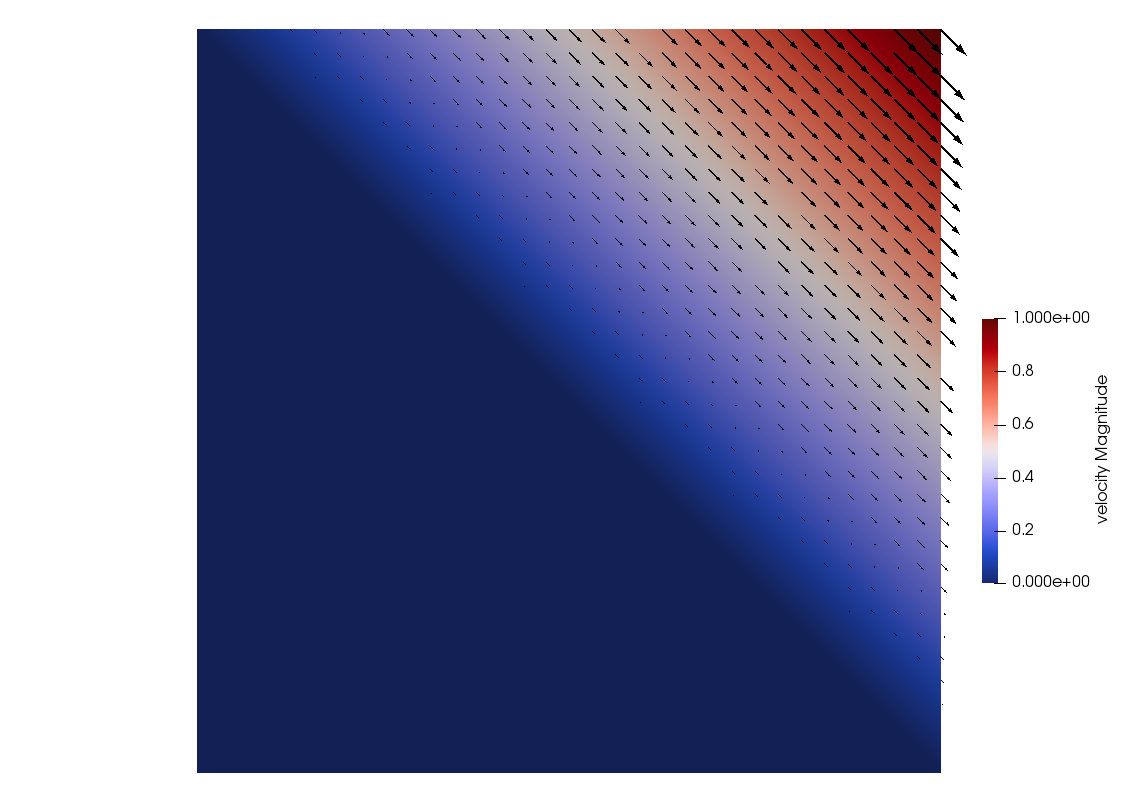
\includegraphics[width=7cm]{python_codes/fieldstone_30/results_couette/vel}\\
{\captionfont 32x32 $Q_1$ mesh}
\end{center}

\begin{center}
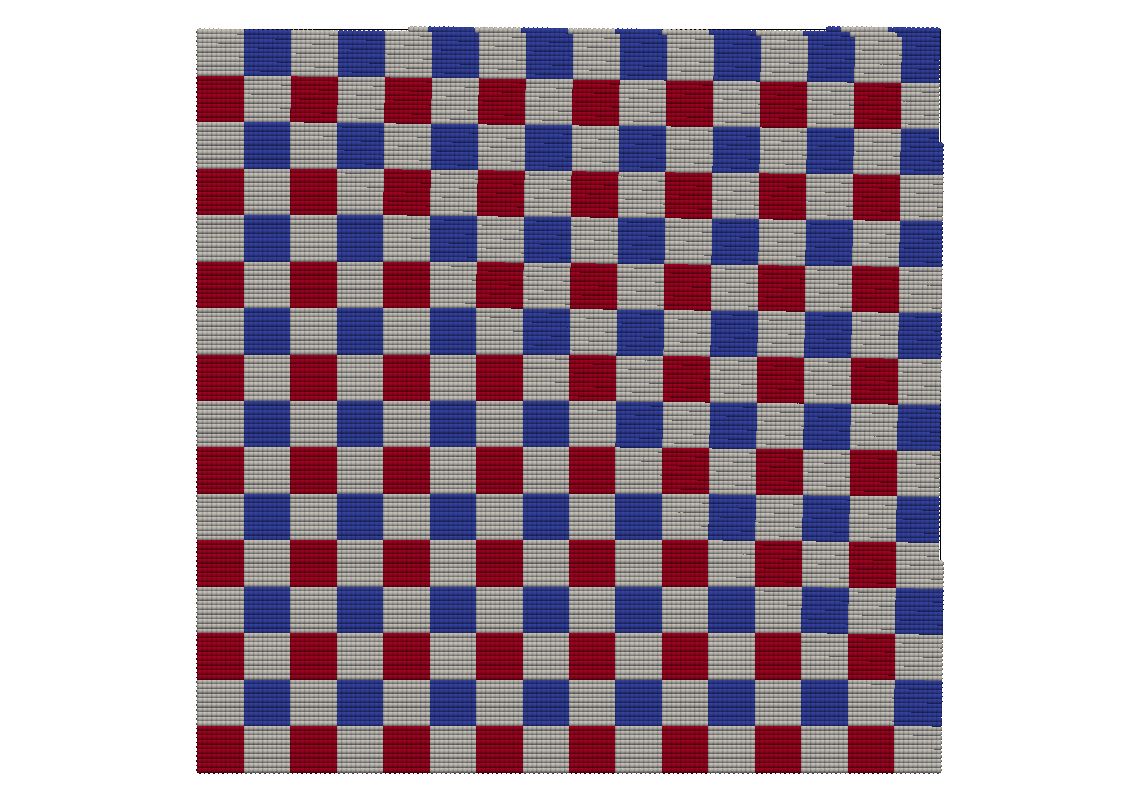
\includegraphics[width=4cm]{python_codes/fieldstone_30/results_couette/particles0000}
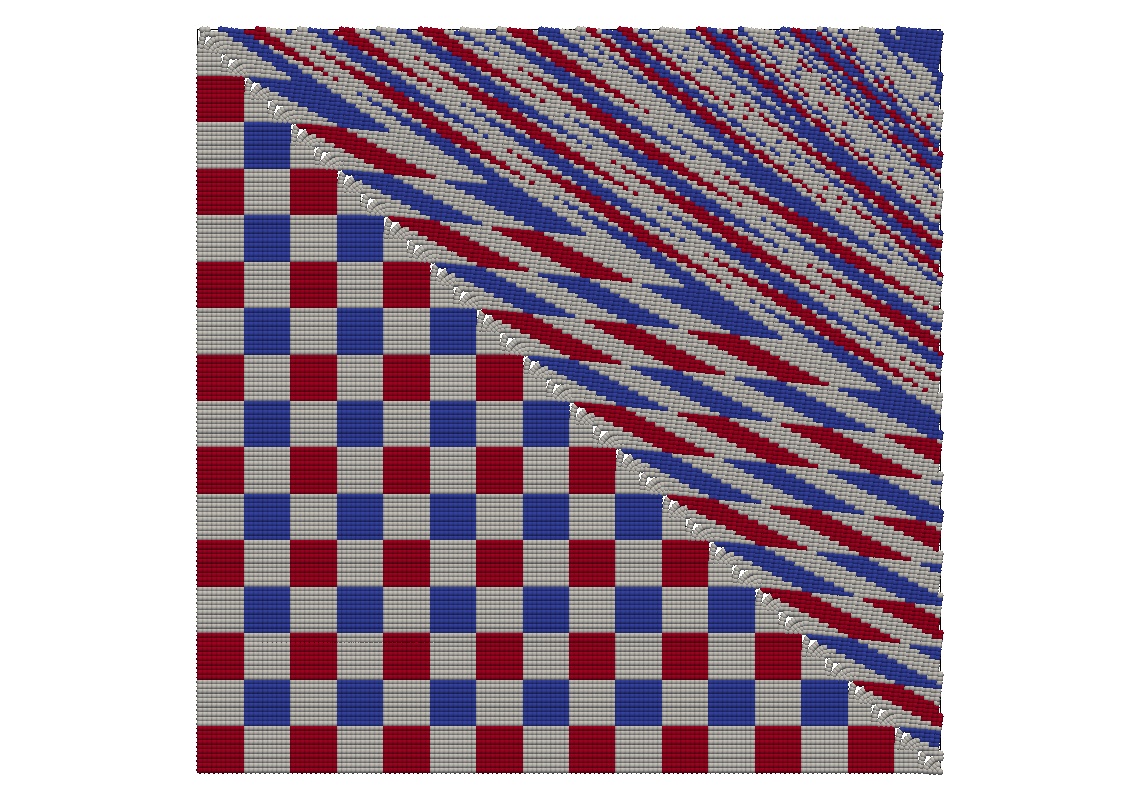
\includegraphics[width=4cm]{python_codes/fieldstone_30/results_couette/particles0010}
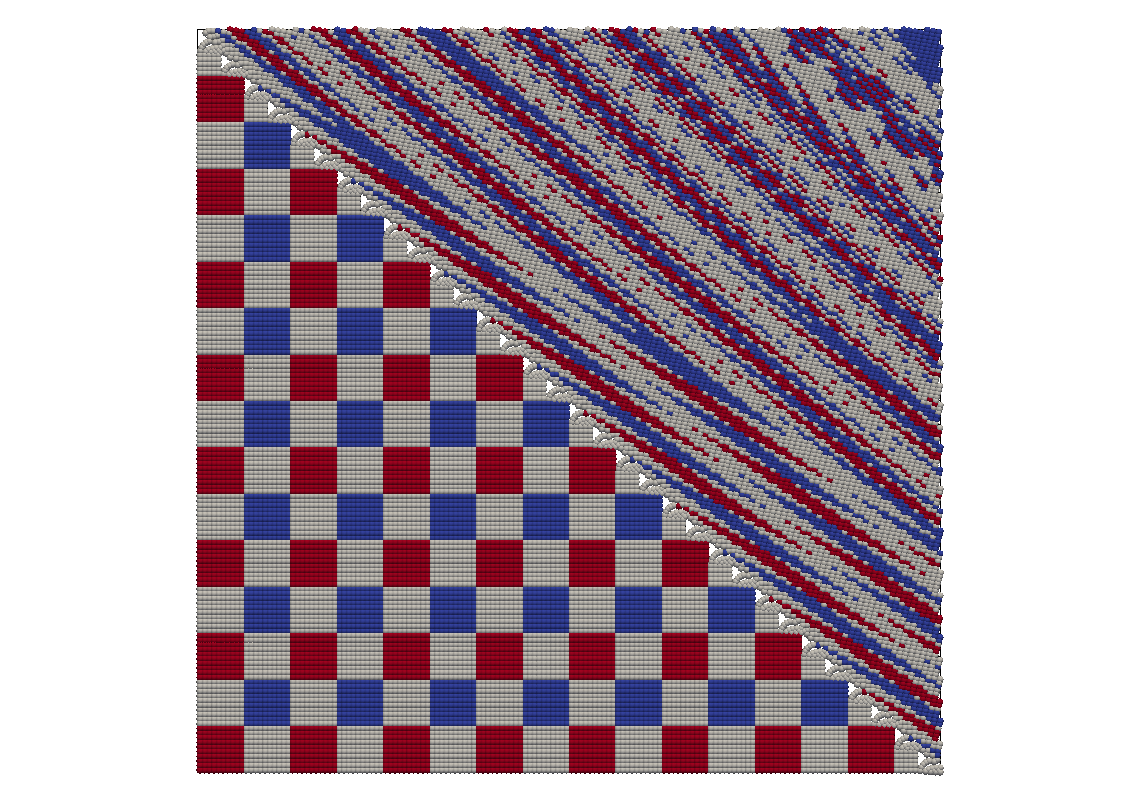
\includegraphics[width=4cm]{python_codes/fieldstone_30/results_couette/particles0020}\\
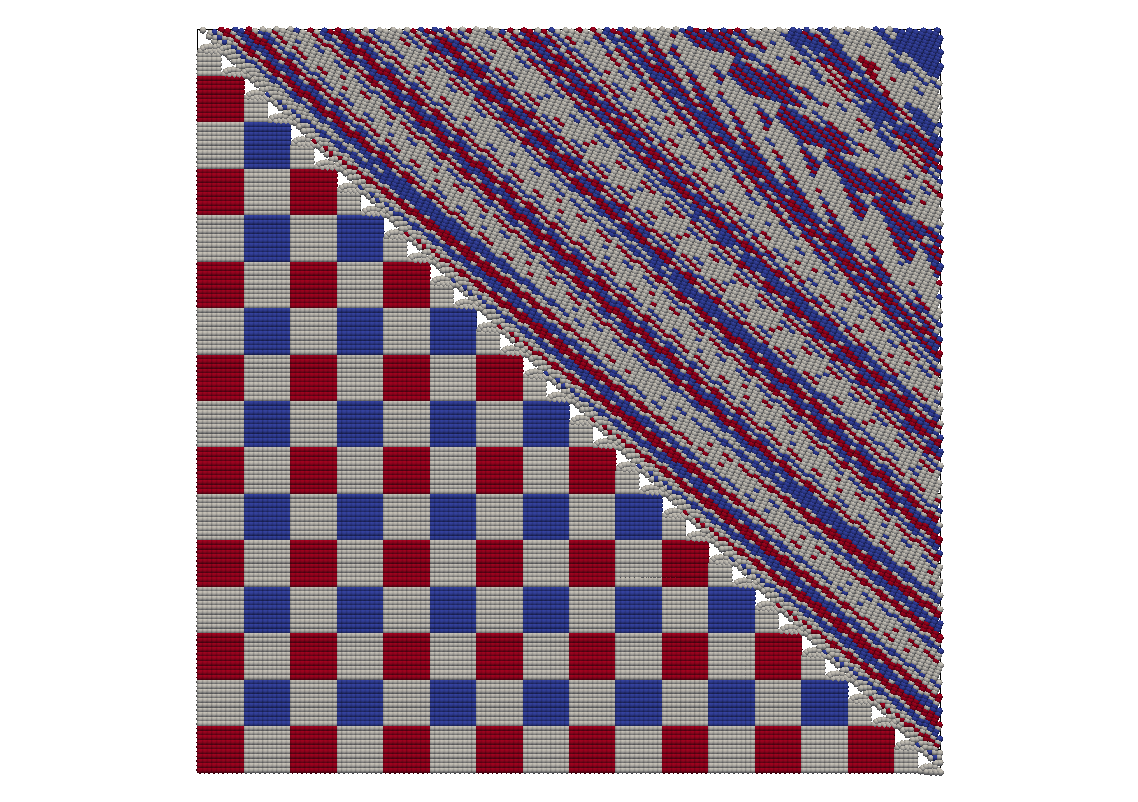
\includegraphics[width=4cm]{python_codes/fieldstone_30/results_couette/particles0030}
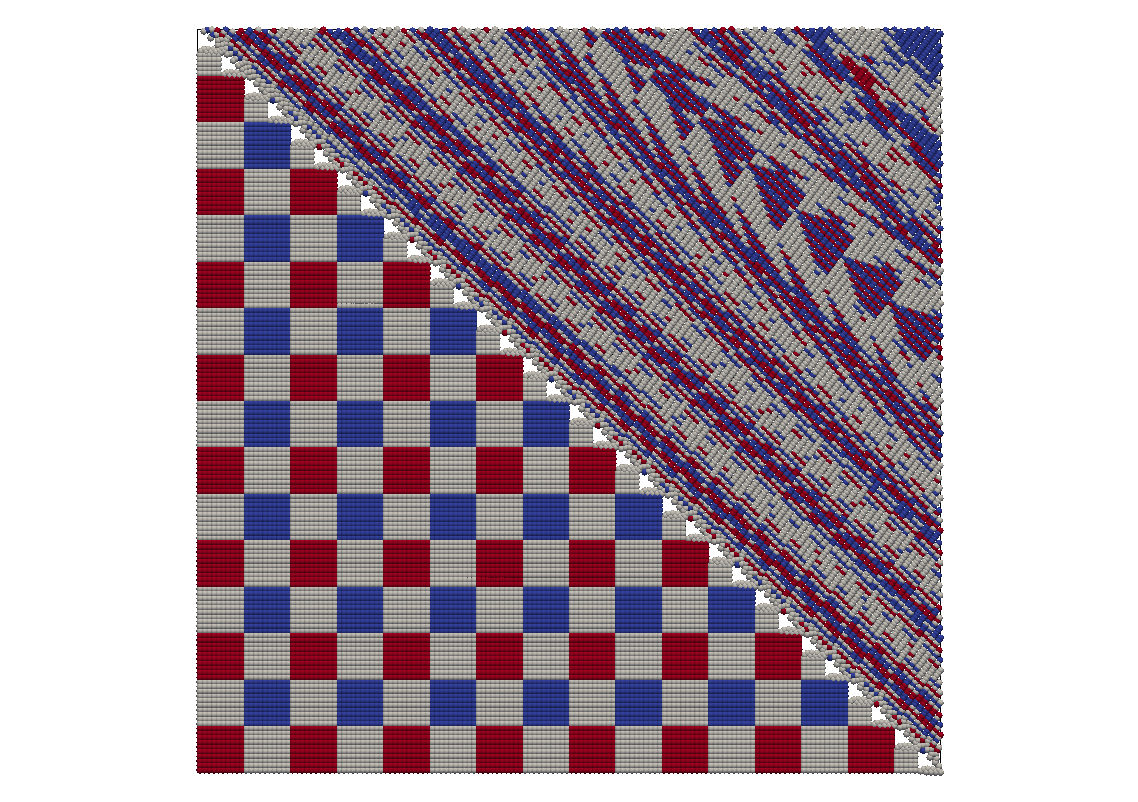
\includegraphics[width=4cm]{python_codes/fieldstone_30/results_couette/particles0040}
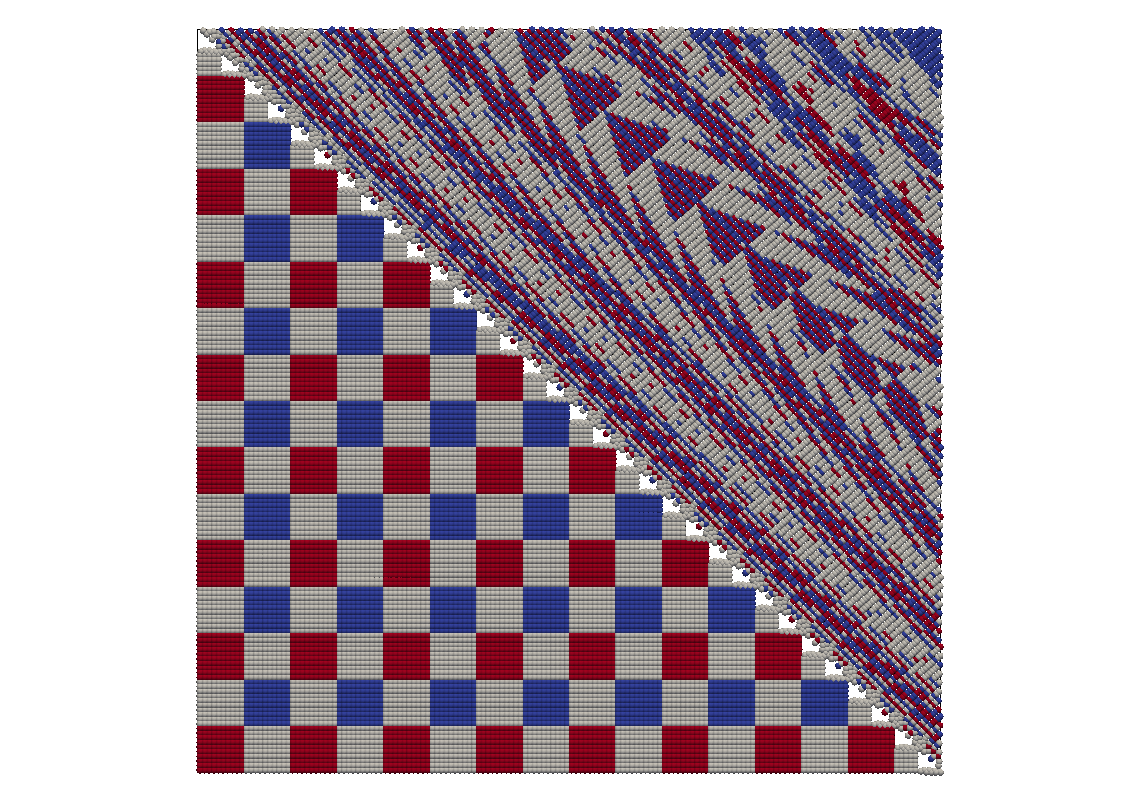
\includegraphics[width=4cm]{python_codes/fieldstone_30/results_couette/particles0050}
\end{center}

Only works with RKorder=1

\newpage
%%%%%%%%%%%%%%%%%%%%%%%%%%%%%%%5
\subsection*{SolCx}

Reference model: 32x32 resolution, CFL nb=0.5, $5^2$ particles randomly distributed inside each 
element, RKorder=2, $Q_1$ interpolation, no cvi.
We look at the min/max number of particles per element as a function of time (normalised 
by the initial number). Total of 250 time steps.

\begin{center}
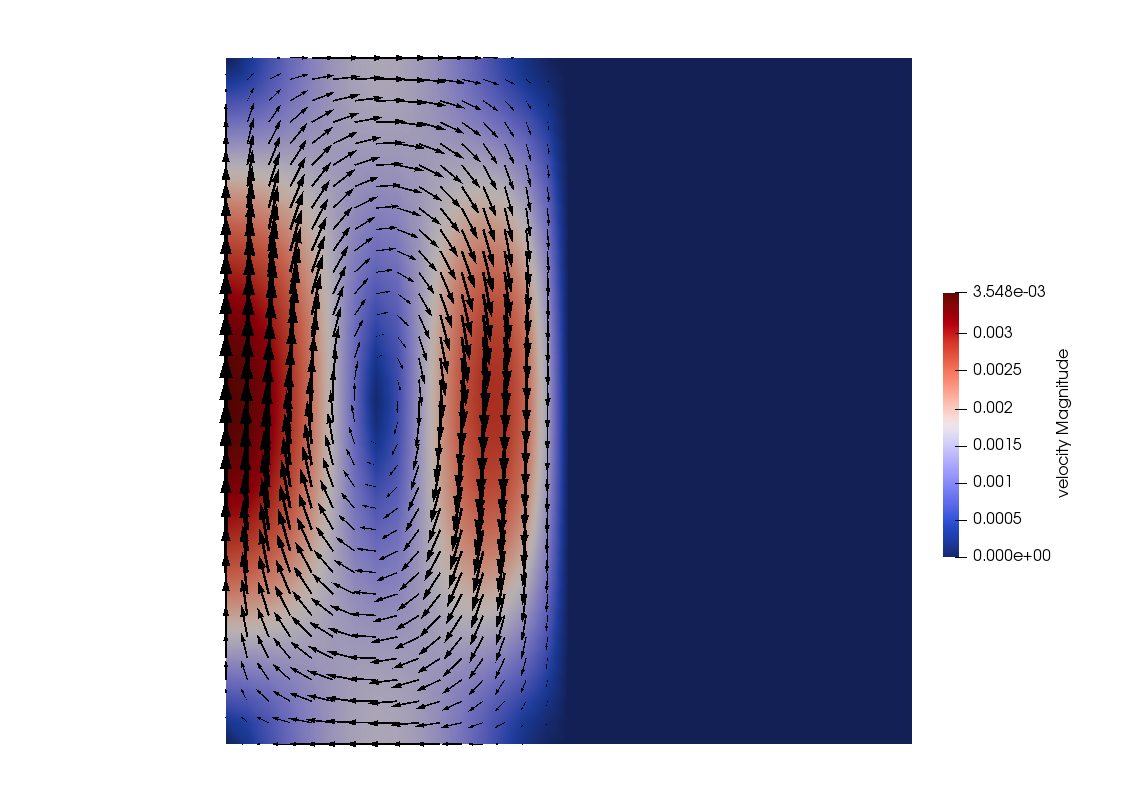
\includegraphics[width=7cm]{python_codes/fieldstone_30/results_solcx/vel}\\
{\captionfont 32x32 $Q_1$ mesh}
\end{center}

\begin{center}
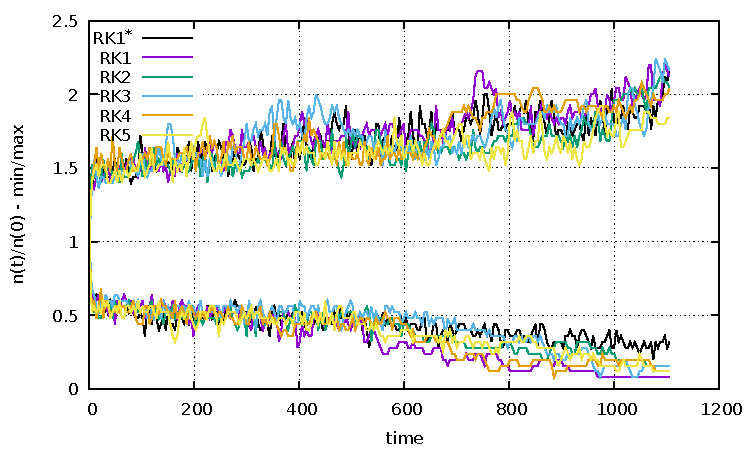
\includegraphics[width=7cm]{python_codes/fieldstone_30/results_solcx/markercount_rk12345}
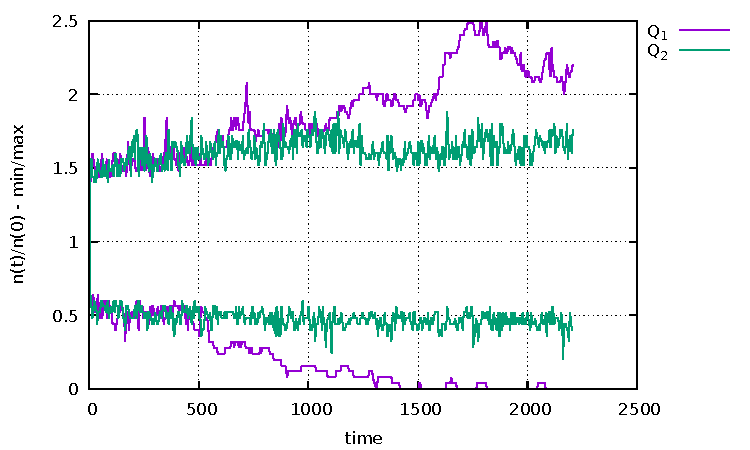
\includegraphics[width=7cm]{python_codes/fieldstone_30/results_solcx/markercount_q12}\\
{\captionfont Left: Ref model + varying RKorder (the star means that velocity 
is directly computed on the particle, no interp.). Right: Ref model + $Q_1$ vs $Q_2$. }
\end{center}


\begin{center}
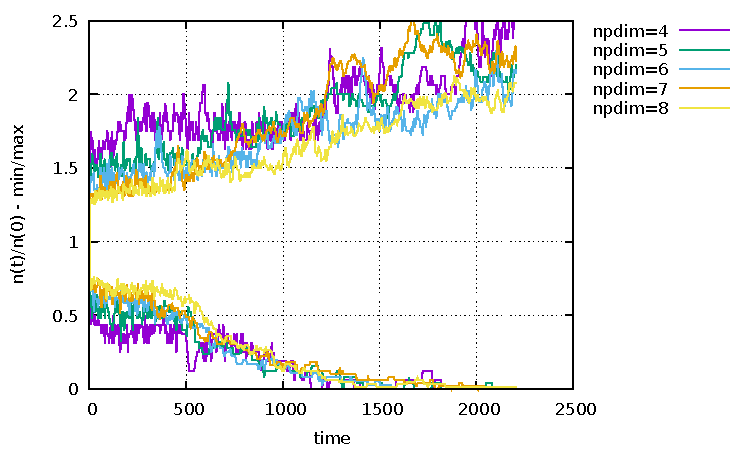
\includegraphics[width=7cm]{python_codes/fieldstone_30/results_solcx/markercount_npd}
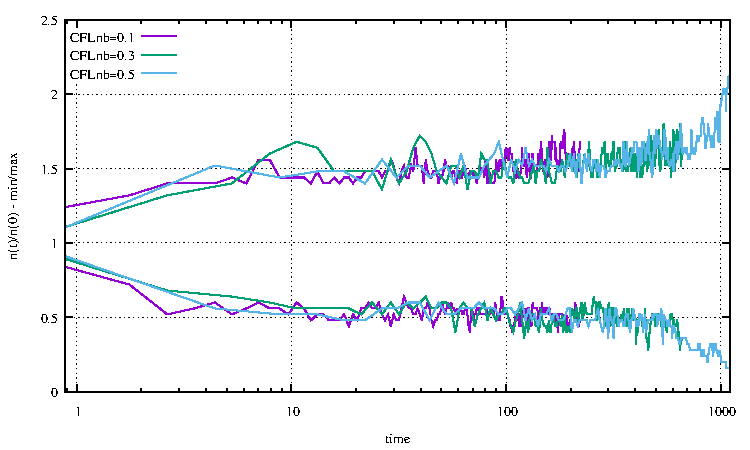
\includegraphics[width=7cm]{python_codes/fieldstone_30/results_solcx/markercount_cflnb}\\
{\captionfont Left: Ref model + initial nparticle per element between 4 and 8. Right: Ref model + CFL nb}
\end{center}

\begin{center}
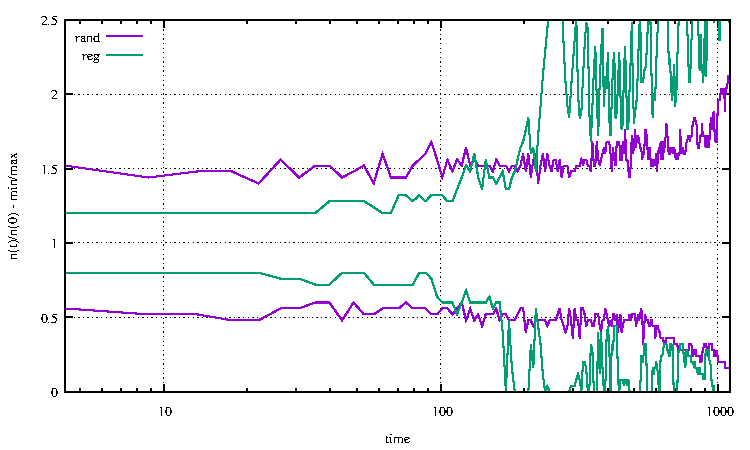
\includegraphics[width=7cm]{python_codes/fieldstone_30/results_solcx/markercount_reg}
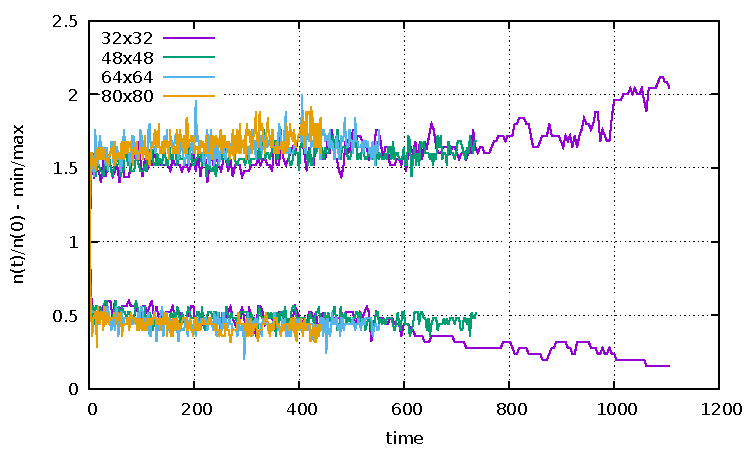
\includegraphics[width=7cm]{python_codes/fieldstone_30/results_solcx/markercount_res}\\
{\captionfont Left: Ref model + random vs regular. Right: Ref model + different resolutions}
\end{center}

Conclusion: nothing really helps, it is a matter of time before an element is fully depleted of particles. 
A regular distribution of markers makes things worse. Only using $Q_2$ interpolation seems to really do 
something. Using a small CFL number will improve things, but at the expense of the calculation walltime. 

\newpage
%%%%%%%%%%%%%%%%%%%%%%%%%%%%%%%5
\subsection*{Streamline flow}


\begin{center}
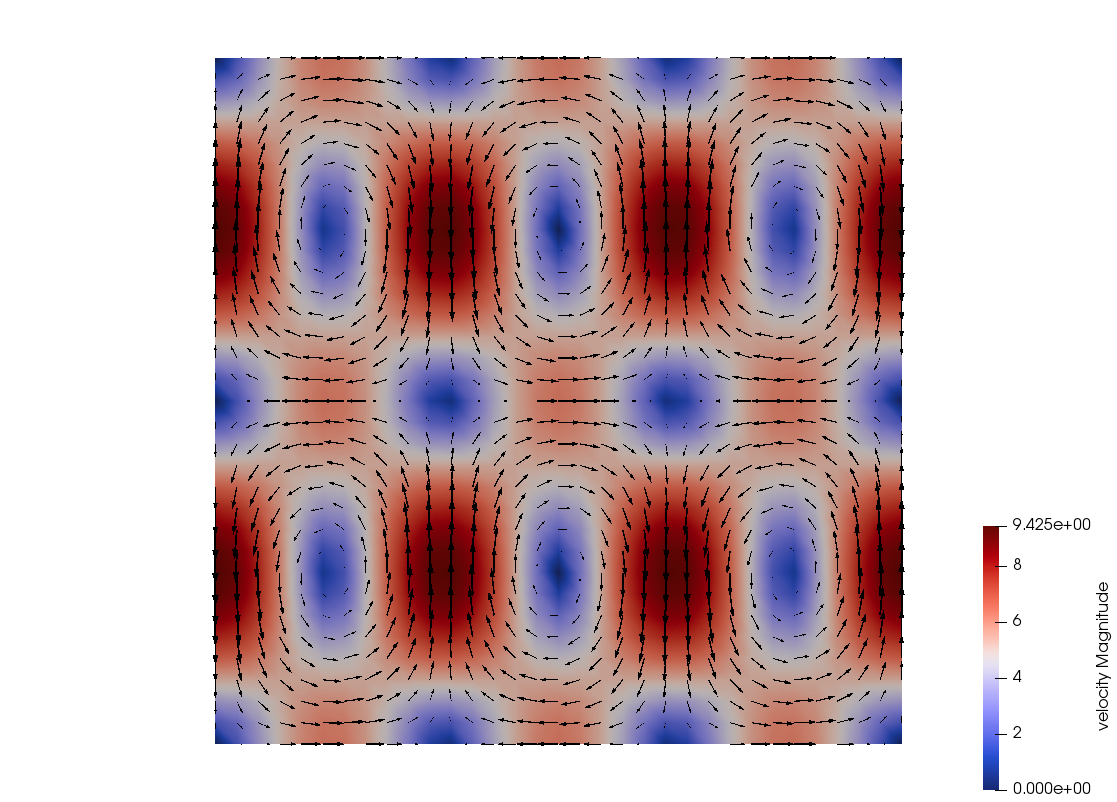
\includegraphics[width=8cm]{python_codes/fieldstone_30/results_streamline/vel}\\
{\captionfont 32x32 $Q_1$ mesh, 3x2 cells}
\end{center}

The reference model is as follows: 32x32 $Q_1$ elements, initial $5^2$ particles per element placed at random, 
CFL number of 0.5, RK order of 2, no CVI.
The {\tt count} array of length {\tt nel} is used to keep track of the number of particles per element. 
Its min/max values over time are recorded. The standard deviation of the {\tt count} array is also 
computed at each time step, normalised by the 
initial number of particles in the element at $t=0$ and plotted as a function of time. 

\begin{center}
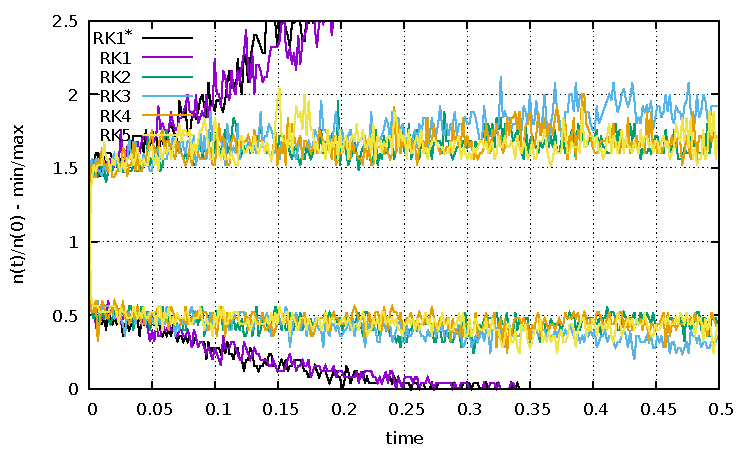
\includegraphics[width=8cm]{python_codes/fieldstone_30/results_streamline/markercount_rk12345}
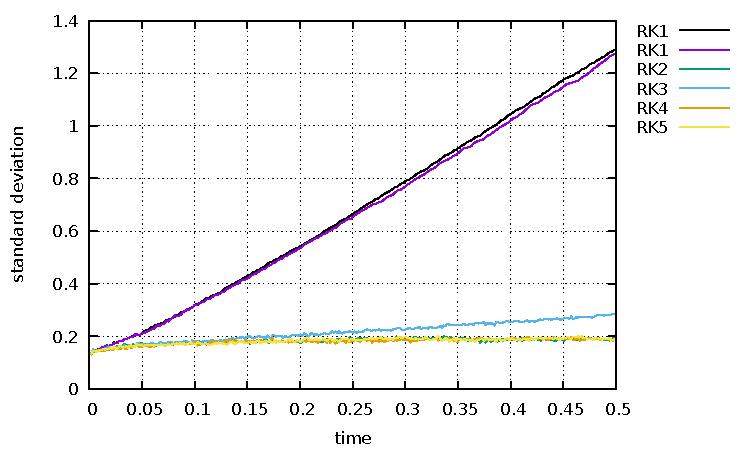
\includegraphics[width=8cm]{python_codes/fieldstone_30/results_streamline/stdev_rk12345}\\
{\captionfont Ref model + varying RKorder (the star means that velocity 
is directly computed on the particle, no interpolation).}
\end{center} 


\begin{center}
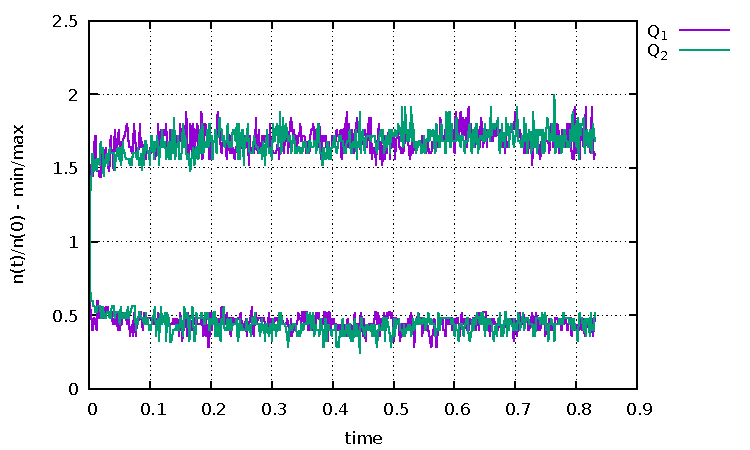
\includegraphics[width=8cm]{python_codes/fieldstone_30/results_streamline/markercount_q12}
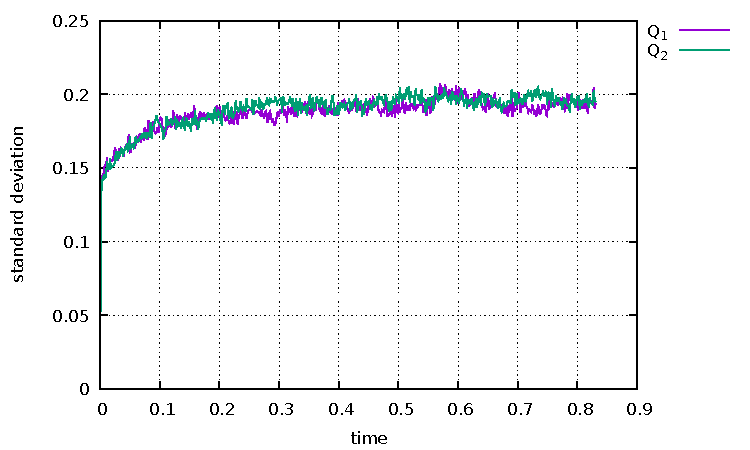
\includegraphics[width=8cm]{python_codes/fieldstone_30/results_streamline/stdev_q12}\\
{\captionfont Ref model + $Q_1$ vs $Q_2$. }
\end{center}

\begin{center}
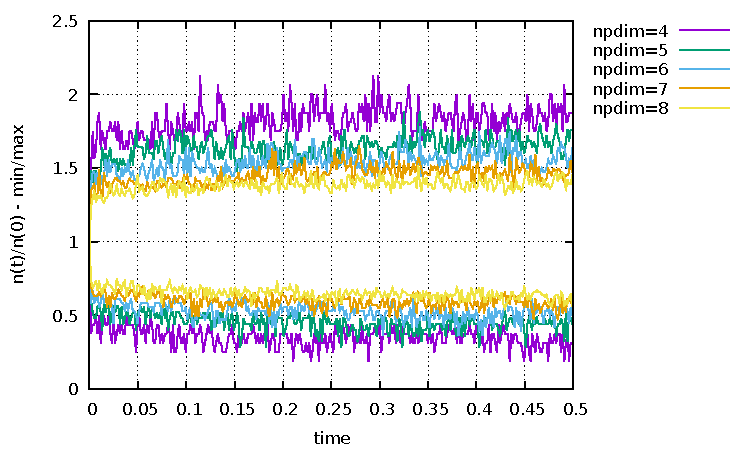
\includegraphics[width=8cm]{python_codes/fieldstone_30/results_streamline/markercount_npd}
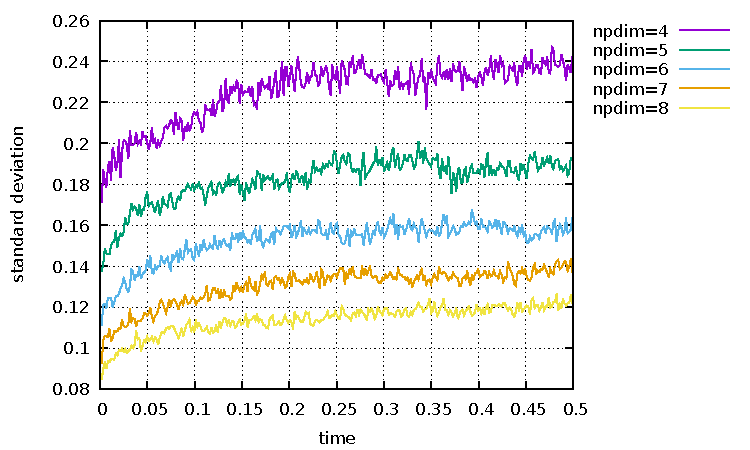
\includegraphics[width=8cm]{python_codes/fieldstone_30/results_streamline/stdev_npd}\\
{\captionfont Ref model + initial nparticle per element between 4 and 8.}
\end{center}

\begin{center}
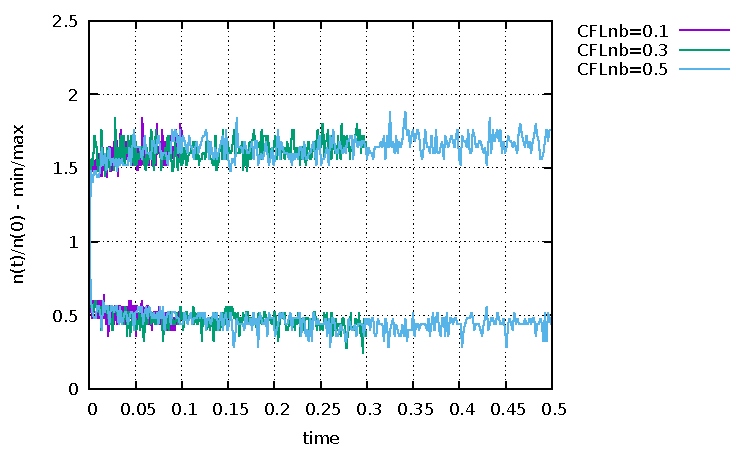
\includegraphics[width=8cm]{python_codes/fieldstone_30/results_streamline/markercount_cflnb}
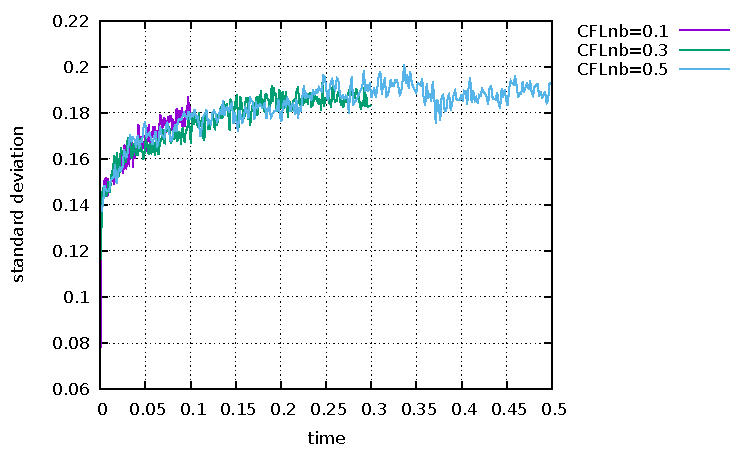
\includegraphics[width=8cm]{python_codes/fieldstone_30/results_streamline/stdev_cflnb}\\
{\captionfont Ref model + CFL nb}
\end{center}

\begin{center}
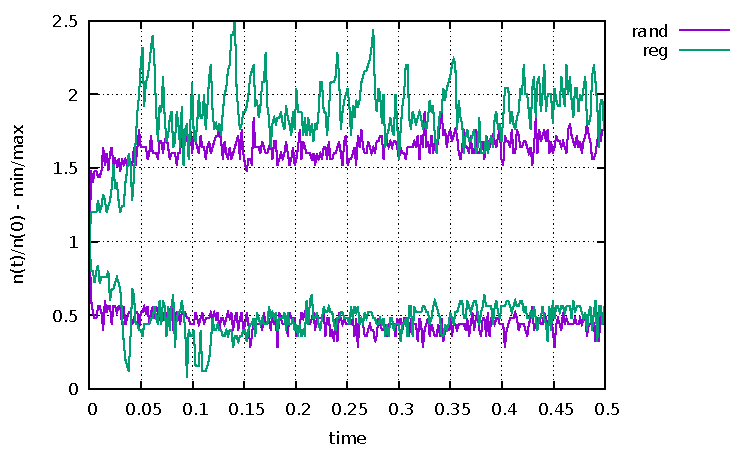
\includegraphics[width=8cm]{python_codes/fieldstone_30/results_streamline/markercount_reg}
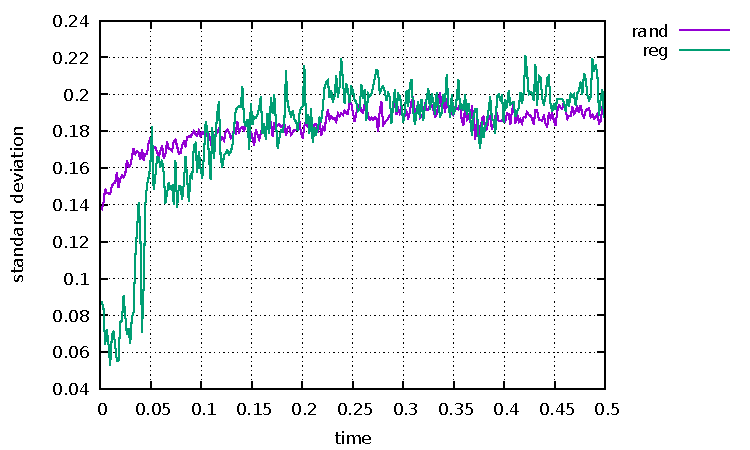
\includegraphics[width=8cm]{python_codes/fieldstone_30/results_streamline/stdev_reg}\\
{\captionfont Ref model + random vs regular.} 
\end{center}

\begin{center}
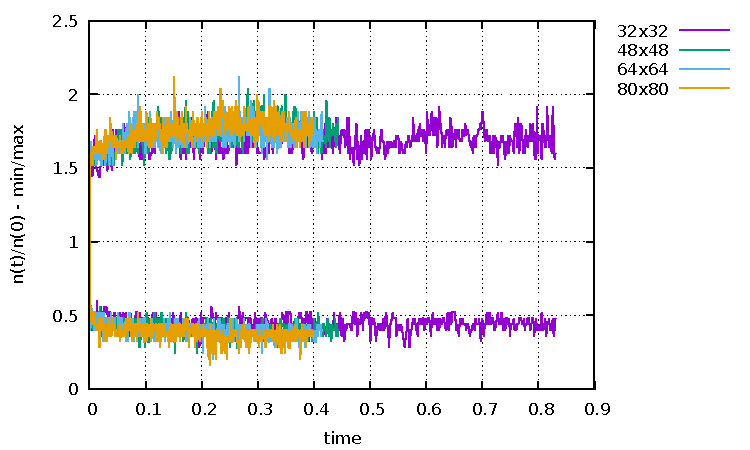
\includegraphics[width=8cm]{python_codes/fieldstone_30/results_streamline/markercount_res}
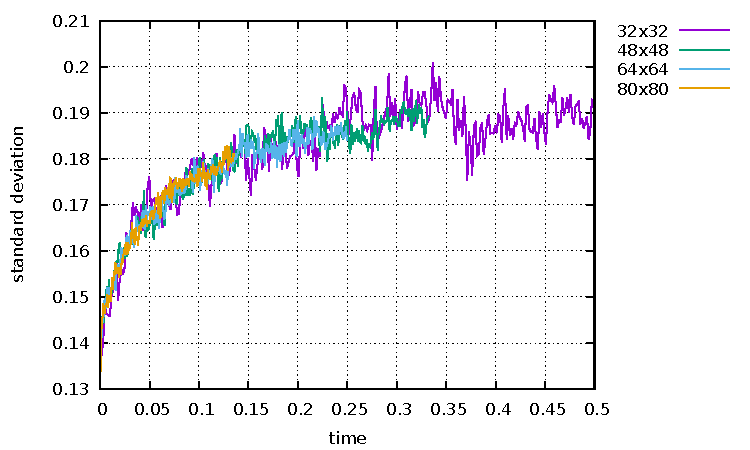
\includegraphics[width=8cm]{python_codes/fieldstone_30/results_streamline/stdev_res}\\
{\captionfont Ref model + different resolutions}
\end{center}








